\documentclass[22pt]{beamer}
\usepackage[orientation=portrait, size=custom, width=121.92, height=91.44,scale=1.35]{beamerposter} % 36in*2.5 = 90cm
\usepackage[absolute,overlay]{textpos}
\usepackage{bookmark} %pdflatex says to use this to avoid errors...
\usepackage{graphicx} %for including images
\graphicspath{{figs/}} %location of images
\usepackage{wrapfig} %wrap text around the images
\usepackage{listingsutf8}    %package for code environment; use this instead of verbatim to get automatic line break; use this instead of listings to get (•)
\usepackage{amsmath}
\usepackage{gensymb}
\usepackage[export]{adjustbox}
\usepackage[skins,theorems]{tcolorbox}
\usepackage{tikz}
\usepackage{multicol}
\newcommand*\circled[1]{\tikz[baseline=(char.base)]{
            \node[shape=circle,draw,inner sep=2pt] (char) {#1};}}
\usepackage{array}
\usepackage{booktabs,adjustbox}
\usepackage{subcaption}
\usepackage{pgfplots}
%plot options
\pgfplotsset{width=7cm,compat=1.8}
\PassOptionsToPackage{gray}{xcolor}

\usetikzlibrary{shapes,shapes.geometric,arrows,fit,calc,positioning,automata}

\usepackage{rotating}
\usepackage{wrapfig}
\usepackage[defernumbers=true,backend=biber]{biblatex}
\addbibresource{references.bib}

%\mode<presentation>
%this doesn't seem to make any difference; leave for now for trying out
\usetheme{Berlin}
\definecolor{MacBlue}{rgb}{0.10196,0.22353,0.53725}
\definecolor{MacMaroon} {rgb}{0.47843, 0, 0.23137}
\definecolor{MacMaroon2} {rgb}{0.47451, 0, 0}
\definecolor{MacGray}{rgb}{0.50196,0.49804,0.51765}
\definecolor{MacMaroon3}{rgb}{00.47,0.2,0.31}
\definecolor{MacGold}{rgb}{1, 0.75,0.35}
\usecolortheme[named=MacMaroon2]{structure}
\setbeamertemplate{caption}[numbered]
\setbeamertemplate{navigation symbols}{}

\def\code#1{\texttt{#1}}

\title{MobilityAI: A Tool for Classifying Human Movements using Machine Learning}
\subtitle{}  %probably want a better subtitle
  \author[Gunasekara, Temelkovski, Tran, Voinea, Hao \& Zheng]{Pasindu Gunasekara, Roberto Temelkovski, Rebecca Tran, Teodor Voinea, supervised by  Dr. Rong Zheng$^\dagger$, Yujiao Hao in collaboration with Dr. Mylinh Duong from Juravinski Hospital \vspace{0.3cm} \newline \small \{gunasepi, temelkr, tranr5, voineat, rzheng, haoy21, duongmy\}@mcmaster.ca}
  \institute[McMaster University]{$^\dagger$Department of Computing and Software, McMaster University \quad \texttt{https://www.eng.mcmaster.ca/cas}\\$^\dagger$Juravinksi Hospital, Hamilton, Ontario}
  \date{December 05, 2018}

\begin{document}
%compile with pdflatex

%there is only one frame, because there is only one page; yeah, it's a posterhttps://www.overleaf.com/project/5bf86bc3f336e22480fff534
%textblock and block seem to work nicely to organize layout
\begin{frame}[fragile]

\begin{textblock}{2}(0.7,1)

\includegraphics[height=8.5cm]{englogo.png} % We can use CAS logo as well? 
\end{textblock}

\begin{textblock}{2}(13,0.2)

\includegraphics[height=17cm,width=20cm]{logo_transparent.png} 
\end{textblock}

\begin{textblock}{9}(4,1)
\titlepage
\end{textblock}

\begin{textblock}{7.25}(0.5,2.9)

\vspace{0.5cm}

%this needs help
\begin{block}{Introduction}
For doctors and nurses at Juravinski Hospital, it is important to be able to accurately assess the effectiveness of existing mobility intervention approaches and discover new strategies to improve efficacy. It is shown that early mobilization and physical therapy is a safe and effective intervention method that can have a significant impact on patient health \cite{adler2012early}. A sensor band will be used to measure mobility data from patients. Machine Learning will then be applied to accelerometer and gyroscope sensor data to accurately determine the actions the sensor band is measuring. The nurses can then use this data to determine how mobile a patient is during their stay compared to their pre-hospitalization mobility levels.

% Although regular check-ins are performed with patients, it can be difficult to be thorough due to the busy schedules of nurses. A solution that can give constant and detailed information about the patient’s mobility would greatly improve the ability for nurses at the hospital to give their patients the care they need. 

%The proposed solution to this problem is to use a clinical %grade wristband that measures movements along with machine %learning to classify movement and body positioning. %Finally, this information is displayed for the hospital %staff to be able to see and interact with through the use %of a mobile application.
\end{block}

\begin{block}{Background}
The following requirements have been developed according to discussions with the doctors from Juravinski hospital:

\begin{itemize}
\item Battery should last and store data for 12 hour shifts
\item Easy to clean, wear and remove
\item Should classify between Standing, Sitting, Lying Down and Walking
\item Software should compare baseline mobility to recorded mobility
\item Software should have an intuitive User Interface
\end{itemize}
\end{block}

\begin{block}{Sensor Band}
Patients will wear the clinical grade wristband, MetaMotionR (MMR), produced by MbientLab with several sensors including a pressure sensor, temperature sensor, and an Inertial Measurement Unit (IMU). The unit is housed in an IP40 case and is strapped on the user with a rubber wrist band.

\begin{figure}
\begin{subfigure}{0.3\textwidth}
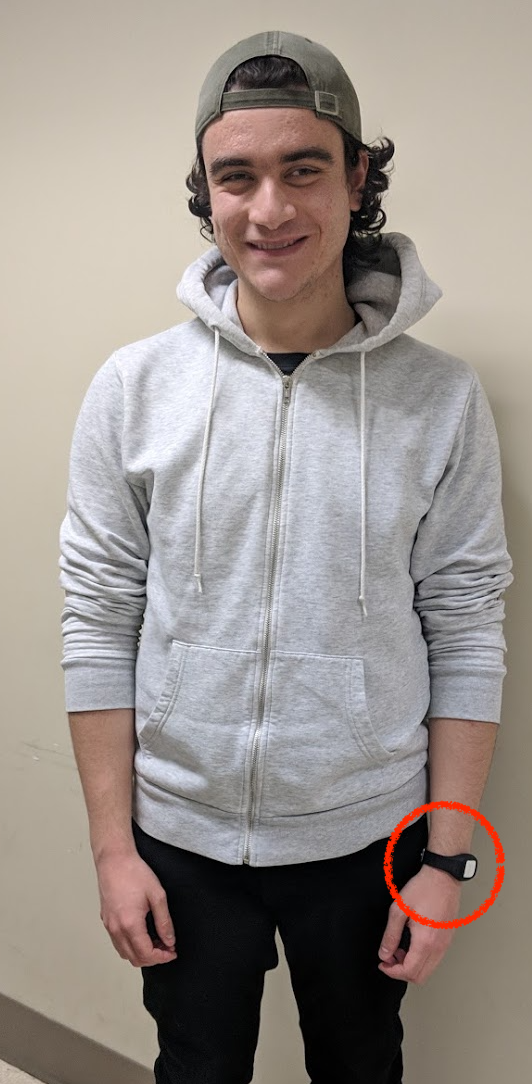
\includegraphics[height=19.2cm,width=12cm]{teo-standing.png}
\end{subfigure}
\begin{subfigure}{0.65\textwidth}
\centerline{\includegraphics[height=10cm,width=12cm]{wristband-teo.jpg}}
\begin{itemize}
\item It contains 8MB of NOR flash memory that can be used to log data, or the device can stream data live using a Bluetooth connection.
\item It also includes a 100 mAH rechargeable battery that can be easily recharged at hospitals using a micro-USB connection
\item The board uses a nRF52 SOC along with Bluetooth Low Energy. 
\end{itemize}

\vspace{1cm}
\end{subfigure}
\begin{subfigure}{0.80\textwidth}
\begin{tabular}{lrrrrr}\label{rawdata}
\textbf{epoch (ms)} & \textbf{elapsed (s)} & \textbf{x-axis (deg/s)} & \textbf{y-axis (deg/s)} & \textbf{z-axis (deg/s)} \\
1542836651794	& 0	& 0.976	& 0.549	& 0.183\\
%1542836651794	& 0	& 0.854	& -0.244	& 0.244\\
%1542836651794	& 0	& 0.793	& 0.305	& 0.244\\
%1542836651939	& 0.145	& 0.61	& 0.366	& 0\\
%1542836651939	& 0.145	& 0.244	& 0.427	& -0.427\\
%1542836651939	& 0.145	& 0.122	& 0.427	& -0.671\\
1542836652055	& 0.261	& 0.122	& 0.244	& -0.549\\
%1542836652055	& 0.261	& 0.183	& 0.366	& -0.305\\
%1542836652165	& 0.371	& 0.305	& 0.366	& -0.122\\
\end{tabular}
\end{subfigure}

\caption{The accelerometer, gyroscope, and IMU will be used to log actions such as walking, sitting, or lying in bed. Each sensor will be sampled 25 times per second and saved to on-board storage. The data will be retrieved using an Android application that will connect to the device when it is nearby. Data will be stored in a CSV format until it can be written to a database.}
\end{figure}

\vspace{-1cm}
\end{block}

\begin{block}{References}
\printbibliography
\end{block}

\end{textblock}

\begin{textblock}{7.25}(8.25,2.9)
\vspace{0.5cm}
\begin{block}{Server and Database Architecture}
The server stores two data sets, accelerometer and gyroscope. It determines when and how the subject is moving.  The data sets are collected through the bands that patients will be wearing.  The Android application will upload this data after it is collected.  The app can request data to display it to the user.

\vspace{1cm}

\begin{subfigure}{1\textwidth}
\vspace{0.3cm}
\begin{subfigure}{1\textwidth}
\centerline{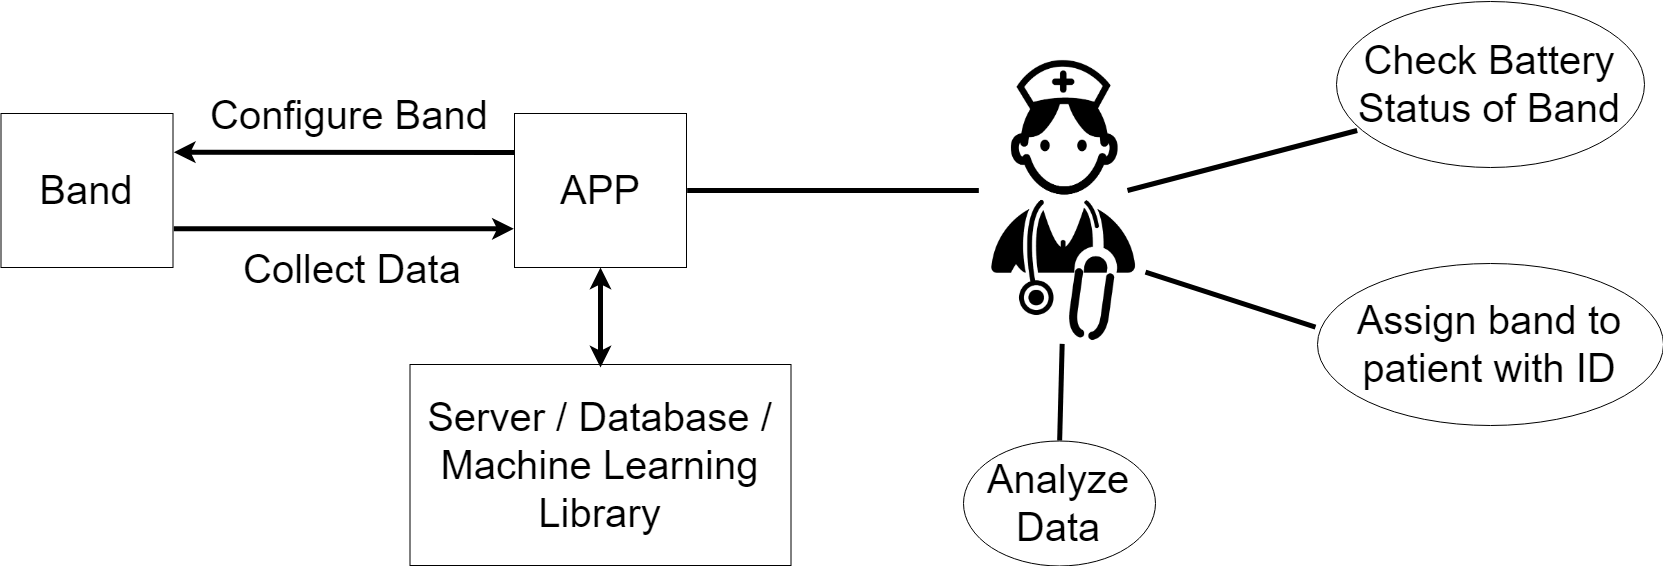
\includegraphics[scale=0.7]{becca_2.png}}
\end{subfigure}\ \ \ \ \
\vspace{2cm}

\begin{subfigure}{1\textwidth}
\centerline{\begin{tabular}{|p{15cm}|p{12cm}|}
     \hline
     \textbf{API Name} & \textbf{API Description}\\
     \hline
     Add Data & Accepts CSV file Writes to database\\
     \hline
     GetRangeAccelerometer GetRangeGyroscope & Retrieves data based on time range\\
     \hline
\end{tabular}}\\
\end{subfigure}
%The application will use the following server API to query %or send data to the database. It calls to \code{AddData}, %which will accept a .CSV file to be written to the %database. The server will be responsible for parsing the %file and writing the rows into the database. Data can also %be queried by start and end times using epoch values of %each row with the \code{GetRangeAccelerometer} or %\code{GetRangeGyroscope} endpoints. Epoch values along with %the MAC address of the device can be used to reference a %patient. Upon request, the database can also return all the %given datasets in the Accelerometer and Gyroscope tables}
\end{subfigure}

%\vspace{0.3cm}
%The tables will consist of seven columns: Id, %Epoch, Timestamp, Elapsed, X-Axis, Y-Axis, and %Z-Axis. The Id is a unique identifier, and the %primary key of both tables. There are two %columns, epoch and timestamp, that are used to %store time. Epoch is the number of milliseconds %that have passed since January 1, 1970, while %timestamp stores the date and time. Epoch is %necessary because it is a single number format, %which allows the Machine Learning tool to parse %through the data easier. Elapsed is the number of %seconds that has passed since the recording began.  

\end{block}


\begin{block}{Machine Learning}
This is a Human Activity Recognition (HAR) problem, and our activity set is defined as follows:

\begin{multicols}{2}
\begin{itemize}
\item Sitting
\item Standing
\item Lying in bed
\item Walking
\end{itemize}
\end{multicols}
The data collection process involves 3 subjects performing each activity for a 2 minute trial, the sampling rate of sensor is 25Hz. The collected dataset is broken down into data frames using a 2.5 second sliding window, starting a new window every 0.5 seconds, allowing for more accurate classification of actions \cite{s100201154}. Each data frame calculated key statistical information such as min, max, average, and variance of x, y, z acceleration and angular velocity.

\begin{figure}
% \begin{tabular}{c|c|c}
%     \textbf{Sensor} & \textbf{Transition Start} & \textbf{Transition Complete}\\
%     \hline
%     \rotatebox[origin=c]{90}{\textbf{Accelerometer}} & \begin{subfigure}{0.45\textwidth}
% \centerline{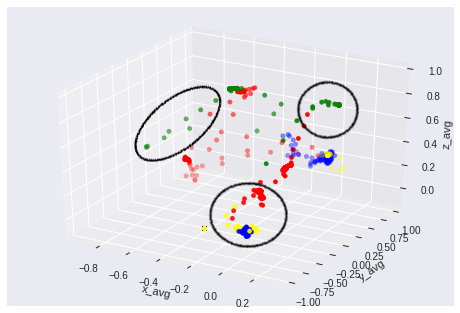
\includegraphics[scale=0.95]{accel_started_diagram.png}}
% \end{subfigure} & \begin{subfigure}{0.45\textwidth}
% \centerline{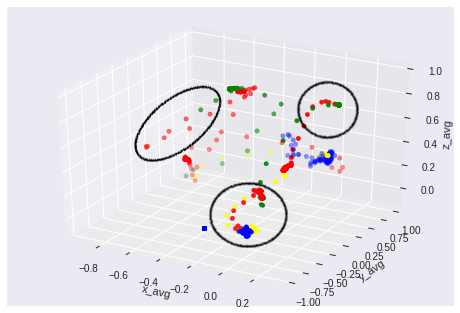
\includegraphics[scale=0.95]{accel_completed.png}}
% \end{subfigure} \\
%     \hline
%     \rotatebox[origin=c]{90}{\textbf{Gyroscope}} & \begin{subfigure}{0.45\textwidth}
% \vspace{0.3cm}
% \centerline{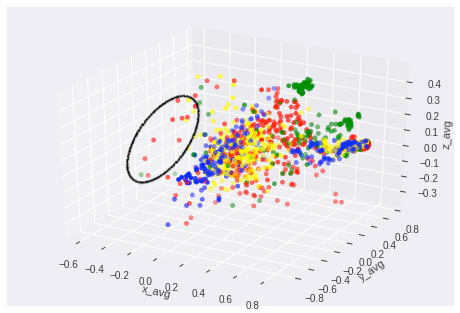
\includegraphics[scale=0.95]{gyro_start.png}}
% \end{subfigure} & \begin{subfigure}{0.45\textwidth}
% \vspace{0.3cm}
% \centerline{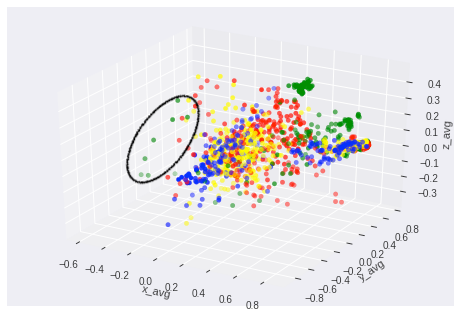
\includegraphics[scale=0.95]{gyro_complete.png}}
% \end{subfigure} \\
% \end{tabular}

\begin{subfigure}{1.0\textwidth}
\centerline{
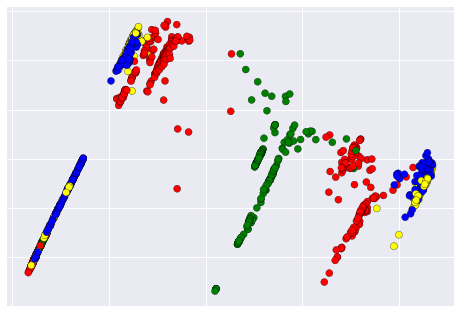
\includegraphics[height=12cm, width=18cm, valign=t]{pca.png}
\hspace{7cm}
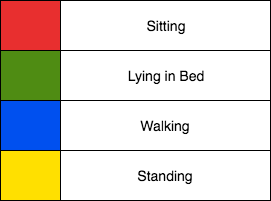
\includegraphics[height=12cm, width=18cm, valign=t]{Chart.png}}
\end{subfigure}

\caption{
Using Principle Component Analysis (PCA), the dataset is reduced from 24 features to 3\cite{scikit-learn}. The 3 features that were selected are those with the greatest proportion of variance, however, due to the nature of PCA, it is unclear which of the original 24 features were chosen. The result of PCA is projected in 2 dimensions in the image above. Each point represents a window. Clusters of like coloured windows can be used to classify future data. There is a strong correlation between the X-Axis values and the action being performed, while the Y-Axis has a smaller effect.}
\end{figure}
\end{block}

\begin{block}{Future Work}
Moving forward with this project, we would like to support new actions such as counting steps and unanticipated actions. Furthermore we would also like to implement live streaming and classification of data from the band.
\end{block}

\end{textblock}

\end{frame}
\end{document}